\documentclass[a4paper]{article}

\usepackage{graphicx}
\usepackage{amsmath,amssymb}
\usepackage{minted}
\usepackage{multirow}
\usepackage{float}
\usepackage{todonotes}
\usepackage{forest}
\usepackage{xstring}
\usepackage{xcolor}
\usepackage[most]{tcolorbox}
\usepackage{xparse}
\usepackage{natbib}

\usetikzlibrary{graphs,graphdrawing}
\usegdlibrary{layered}

% for external graphviz
\input{/home/donkarlo/Dropbox/repo/nd_ai_project/src/nd_ai/knoweldge_representation/language/formal/computer/programming/tex/latex/code_clips/external_graphviz.tex}

% for tags
\input{/home/donkarlo/Dropbox/repo/nd_ai_project/src/nd_ai/knoweldge_representation/language/formal/computer/programming/tex/latex/parts/control_sequence/kinds/semtag/semtag.tex}

% for links
\input{/home/donkarlo/Dropbox/repo/nd_ai_project/src/nd_ai/knoweldge_representation/language/formal/computer/programming/tex/latex/code_clips/seehere.tex}

\title{Cognitive bias}
\date{}

\begin{document}
    \maketitle
    \clickurlfooter{https://en.wikipedia.org/wiki/Cognitive_bias} defines cognitive bias as a systematic pattern of deviation from norm or rationality in judgment.
    
    \begin{figure}[H]
        \centering
        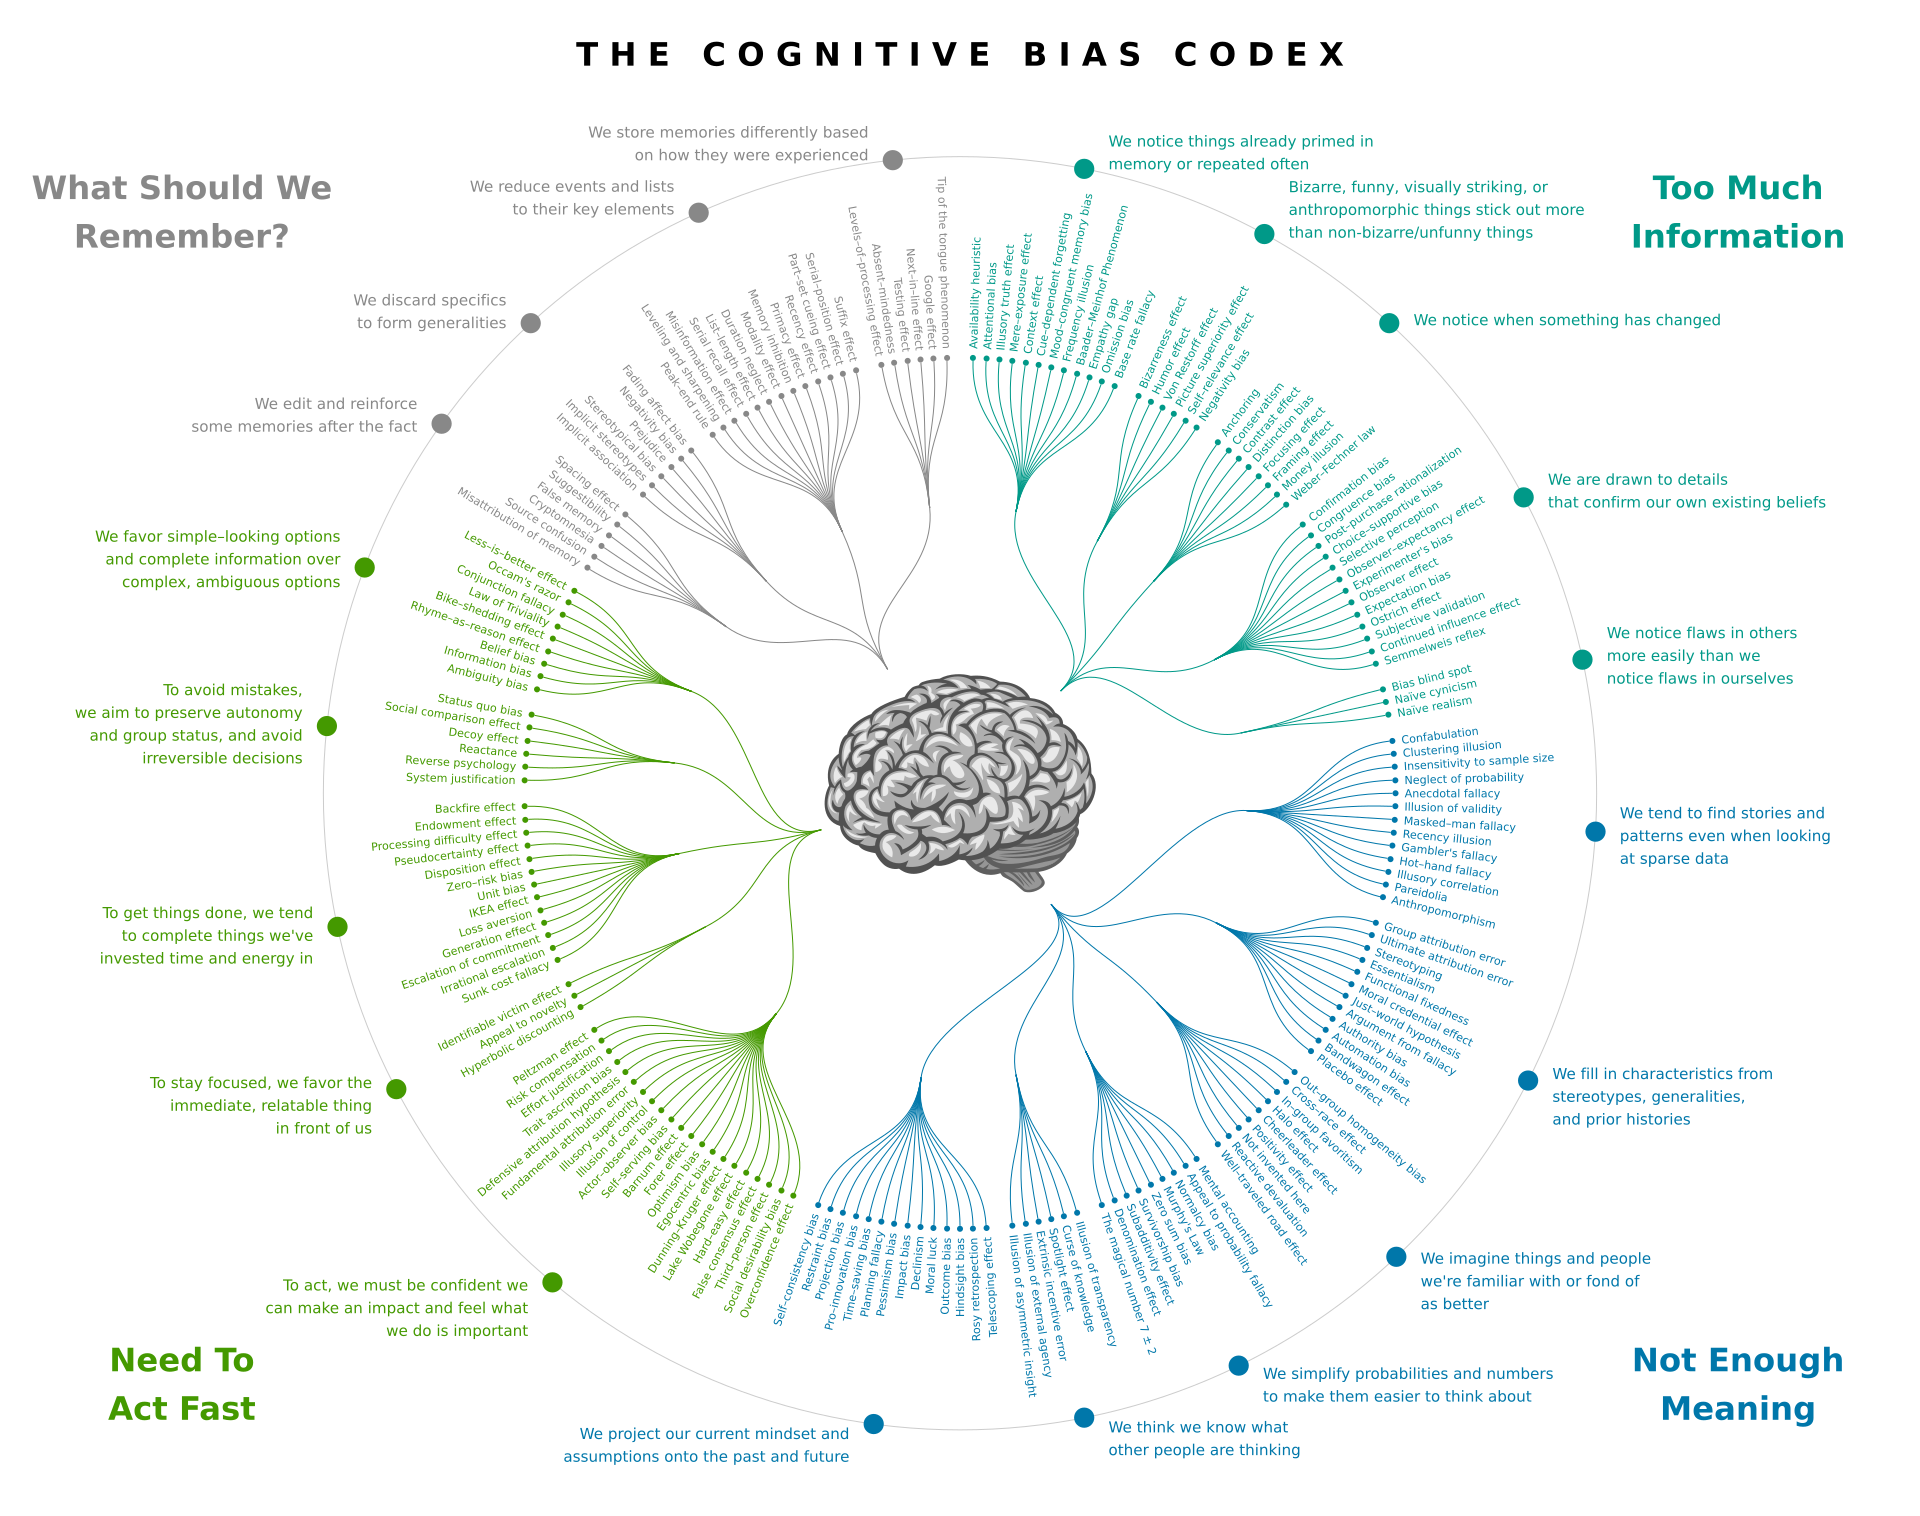
\includegraphics[width=0.9\textwidth]{cognitive_bias_codex.png}
    \end{figure}
    %\bibliographystyle{plainnat}
    %\bibliography{/home/donkarlo/Dropbox/repo/nd_shared_research/bibliography/bibliography.bib}
\end{document}